\chapter{Introduction}


\chapter{Literature Review}

\section{Design of Experiments}
One of the main objectives when performing numerical, or real experiments, is to understand the variation of a Quantity of Interest (QoI) with respect to the variation of some input parameters~\citep{Sacks1989}. Each experiment, or sample, corresponds to a particular set of input parameters $x_k$ with $k \in [1, \dots , d]$, where $d$ is the number of dimensions. As a result, the group of $N_s$ samples, or Design of Experiments (DoE), is noted as $\mathbf{X}^{N_s}_d${\color[rgb]{0.9,0.2,0.16}\footnote{For simplicity either the dimensionality $d$ or the number of sample $N_s$ is omitted. Nevertheless, the subscript denotes $d$ while the superscript denotes $N_s$.}}. Then the forward model (or experiment) $\mathcal{M}$ can be simulated for each sample
\begin{align}
(\mathbf{X}^{N_s}_d, \mathcal{Y})=\left(\mathbf{x}^{(i)},\mathbf{Y}^{(i)}\right)_{1\leq i\leq N_{s}},
\end{align}
\noindent where $\mathcal{Y}$ is the QoI and $\mathbf{Y}^{(i)} := \mathcal{M}(\mathbf{x}^{(i)})$ corresponds to the deterministic integration of the forward model $\mathcal{M}$ as a black box for the $i$th set of input parameters $\mathbf{x}^{(i)}$---see~\cref{fig:doe}.

\begin{figure}[H]
\centering
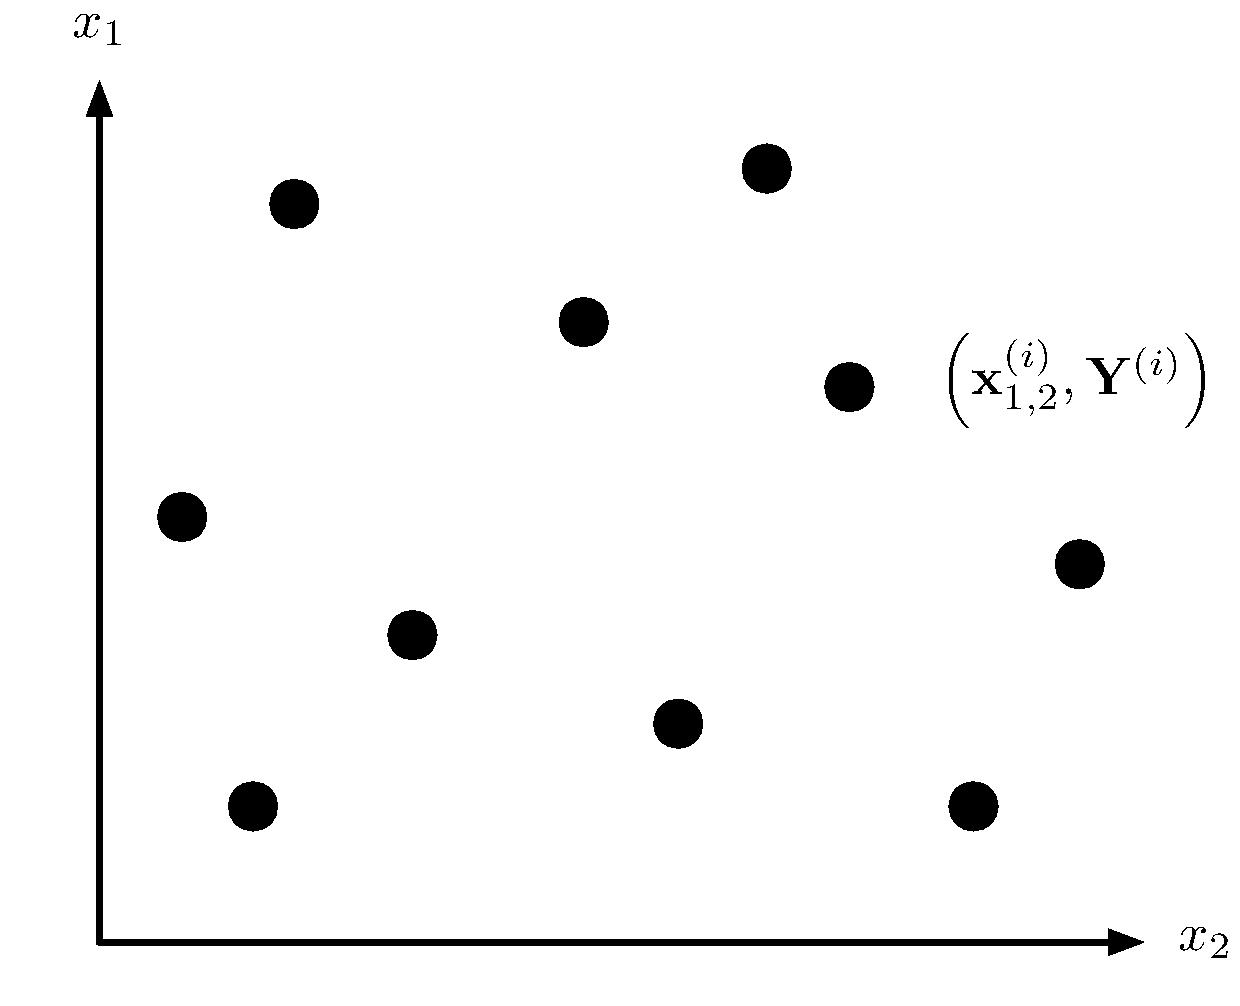
\includegraphics[width=0.5\linewidth,keepaspectratio]{fig/literature/doe.pdf}
\caption{Sketch of a 2-dimensional Design of Experiments.}
\label{fig:doe}
\end{figure}

In its basis form, a DoE is described by a $d$-dimensional cube: a hypercube---see~\cref{fig:hypercube}. A hypercube is parametrised by the minimal and maximal values of each parameters. In case parameters depends on each others, or if there are constrains on the parameters, non-rectangular domains~\citep{Lekivetz2015} have to be considered.

\begin{figure}[H]
\centering
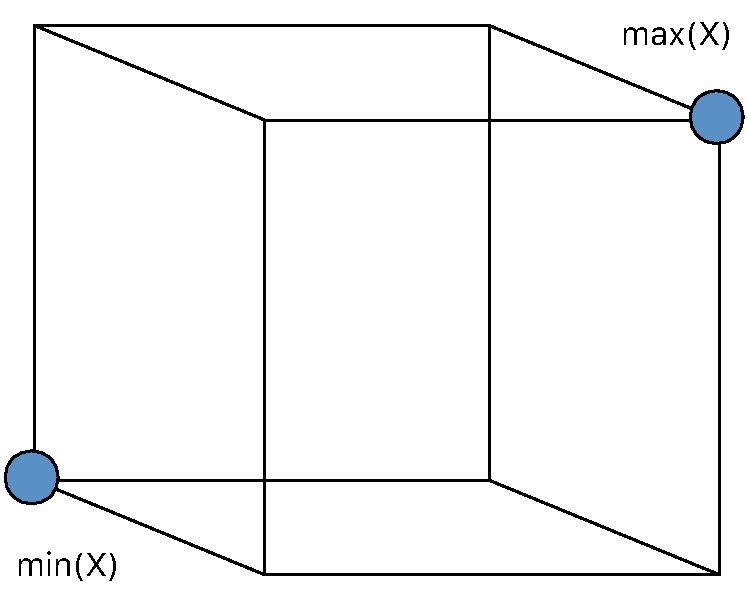
\includegraphics[width=0.5\linewidth,keepaspectratio]{fig/literature/hypercube.pdf}
\caption{Sketch of a 3-dimensional hypercube.}
\label{fig:hypercube}
\end{figure}

From exploratory phases to more advanced analyses, such as Uncertainty Quantification (UQ) and robust optimization, DoE aims at helping better understand the physical mechanisms governing the problem of interest~\citep{Saltelli2007}. Therefore, the objective of efficient DoE is to maximize the coverage of input space, i.e., space filling, with the aspiration of capturing most of the underlying physics. Such analyses typically require large number of experiments in order for the statistics of the QoIs to converge. In this regard, many studies have focused on trying to reduce the computational cost. However, depending on the required quality of the analysis, the complexity of the experiment, or its return time, the total number of experiments may be limited. Thus, the objective is to optimize the space-filling properties for a given budget.

Different metrics are commonly used to assess the space filling of a DoE. They can be categorized into \emph{(i)} geometrical and \emph{(ii)} uniformity criteria. Among the most used geometrical criteria are the \emph{maximin} and \emph{minimax}~\citep{Pronzato2017}. They, respectively, maximize the minimal distance between all points or minimize the maximal distance between any location in space and all points of the sample. A similar criterion is found by using a \emph{minimum spanning tree}~\citep{Franco2009} in which the best design corresponds to a maximization of the mean distance between all connections and the minimization of the variance in these distances. The uniformity criterion, instead, measures how the spread of the points deviates from a uniform distribution. The central discrepancy is commonly used~\citep{Fang2006,Damblin2013} to measure the uniformity.

There are three main methodologies for defining a DoE: \emph{(i)} \emph{Monte Carlo} (MC), \emph{(ii)} \emph{Latin Hypercube Sampling} (LHS) and \emph{(ii)} Quasi-\emph{Monte Carlo} (QMC) methods~\citep{Cavazzuti2013,Garud2017}. Kucherenko \emph{et al.}~\citep{Kucherenko2015} have recently compared MC and LHS against the well-established low discrepancy sequence of \emph{Sobol'}. They concluded that LHS and QMC both offer superior integration performance over MC.

LHS-based sampling methods are one-shot design strategies~\citep{Mckay1979,Fang2006}. Their utilization requires the practitioner to set \emph{a priori} the total number of samples contained in the DoE. Although, there have been some attempts to construct progressive LHS, they still require an initial design to work properly~\citep{Sheikholeslami2017}. On the other hand, low discrepancy sequences are iterative designs which can be continued without compromising the discrepancy. The practitioner is then able to increase the number of samples afterwards for quality reasons, for instance, or if other experiments can be afforded. Liu \emph{et al.}~\citep{Liu2018} recently reviewed iterative DoE in a metamodeling context. In their study, it is shown that most iterative methods need an initial design as a starting point. A particular benefit of this approach is that it allows the use of physics information from the system to guide the DoE. In this case, such iterative methods are called adaptive methods. Except for some work in~\citep{Crombecq2011}, and to the best of the authors’ knowledge, the number of iterative methods not requiring an initial design is limited. This state-of-the-art can be explained both by the quality of the initial designs (using LHS of \emph{Sobol'} sequence) and by the performance of the refinement algorithm. There are even fewer options if the iterative design cannot take advantage of the output of the experiments. Low discrepancy sequences are an example of such methods. But in some context, stochastic methods may be required ---\thinspace to compute sensitivity indices for instance~\citep{Saltelli2010}. Scrambling the sequences~\citep{Owen1998} can avoid this pitfall but then the method is no longer iterative.

\section{Uncertainty Quantification}\label{sec:uq}

\subsection{Uncertainty Propagation}\label{sec:up}
Uncertainty Propagation (UP) seeks to communicate uncertainties throughout the system. Uncertainties are defined at one side of the system, and their effects are observed at the other end. But are we talking about the uncertainties of the input parameters or the output QoI? Usually, uncertainties are defined on the input parameter space side, and it is the impact on the quantity of interest that is observed. The other way around is called an \emph{inverse problem} and is not discussed in this work.

Uncertainties can be described using a probabilistic approach through the use of Probability Density Functions (PDF). Thus, propagating uncertainties comes to determining the PDF of the QoI.

\begin{figure}[H]
\centering
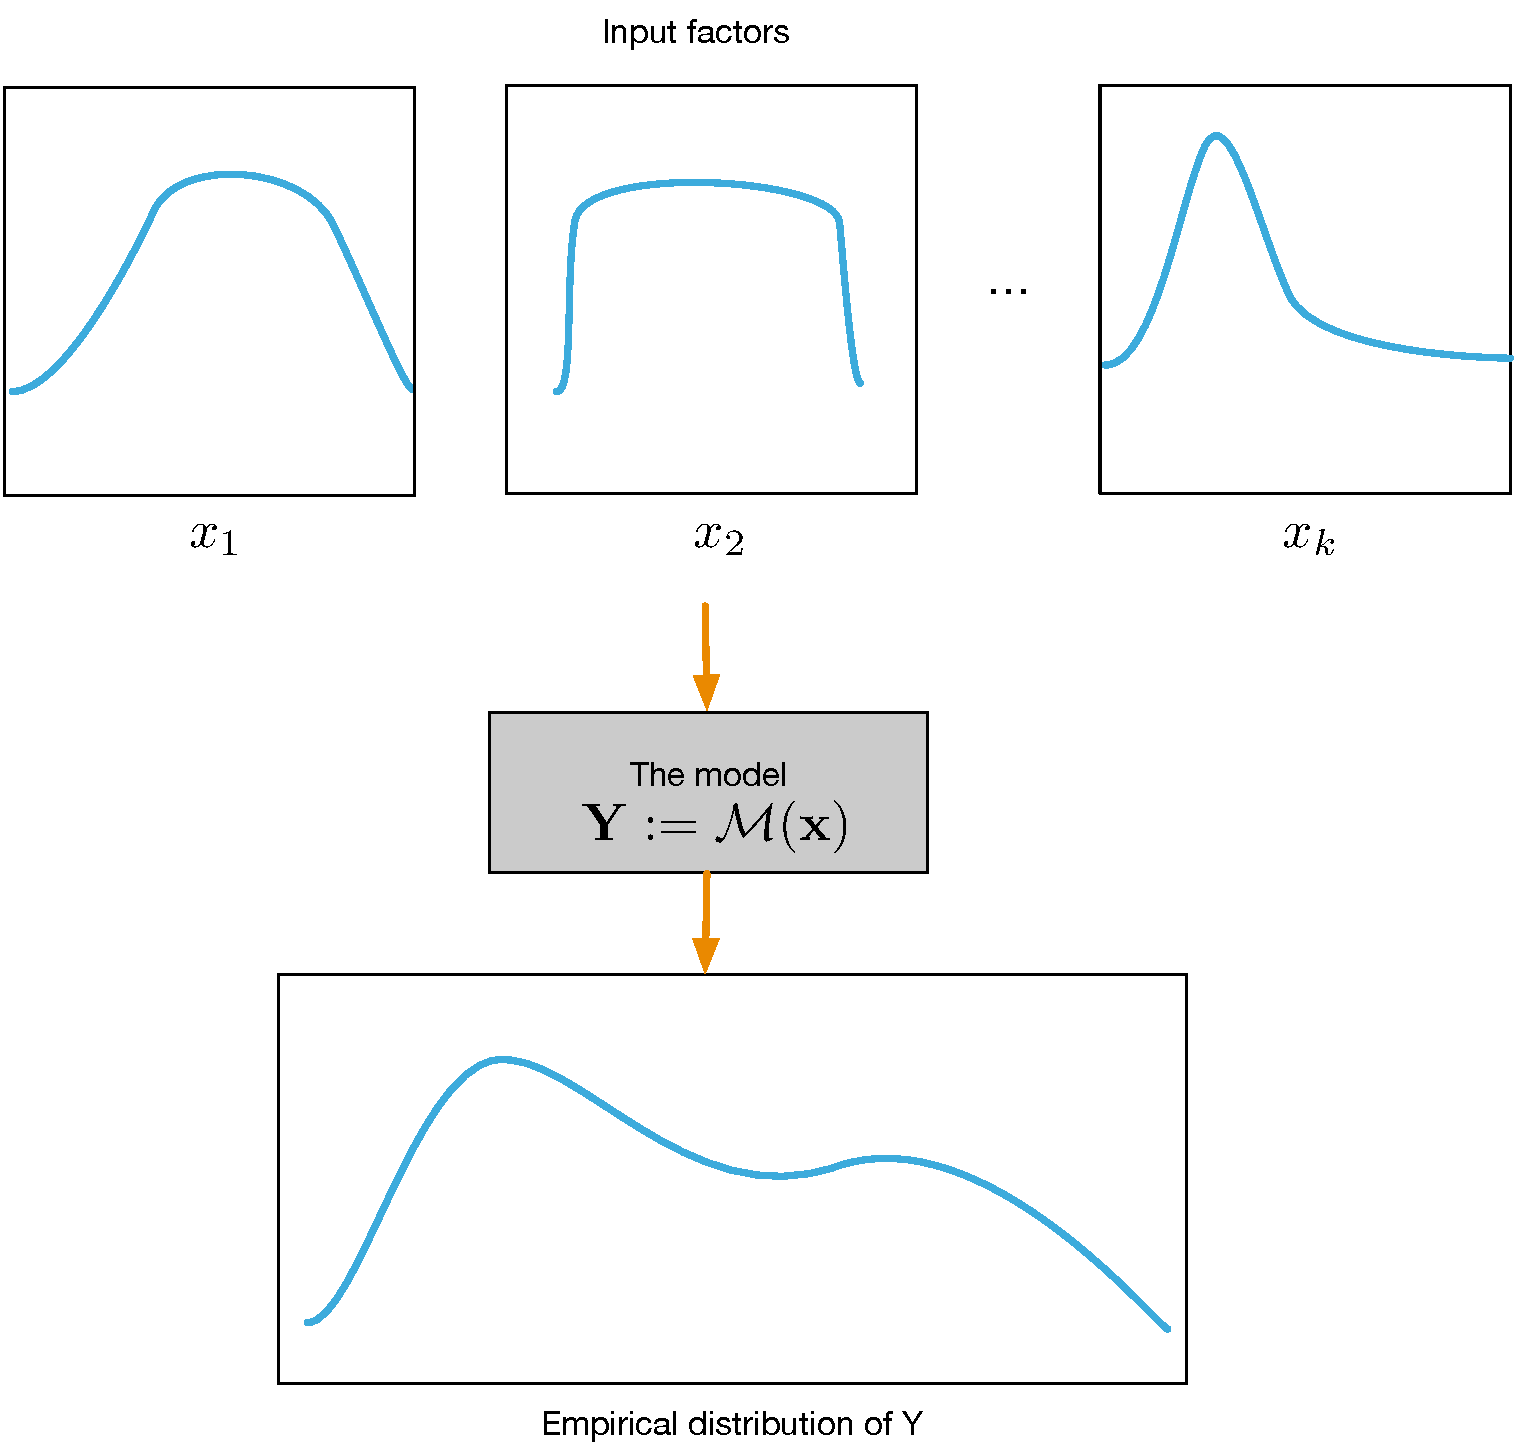
\includegraphics[width=0.7\linewidth,keepaspectratio]{fig/literature/propagation.pdf}
\caption{Sketch of the Uncertainty Propagation procedure.}
\label{fig:UP}
\end{figure}

\Cref{fig:UP} present a representation of the UP procedure. In practice, propagating uncertainties comes to sampling the PDFs of inputs and observing the impact on the QoI. As we are interested in computing statistics on the QoI, this requires a statistically significant sampling. A large number of samples is required to recover the empirical PDF of the QoI. One must note that in order to find the tail of the PDF---the least frequent event---it requires an even larger number of samples.

Histograms can be used to represent the PDF. However, continuous functions can be obtained using a technique called Kernel Density Estimation (KDE)~\cite{Wand1995}. The PDF estimator $\hat{f}(Y^*)$ is given by:
\begin{align}
\hat{f}(Y^*)&= \frac{1}{N_{s}}\sum_{i=1}^{N_{s}} K_{h_i}(Y^*-Y^{(i)}),
\end{align}
\noindent where $N_s$ is the number of samples and $K_{h_i}(.) = K(./h_i)/h_i$ is the scaled kernel chosen for the modal probability density function with $h_{i}$ the bandwidth for the \emph{i}th component. In the present work $K$ is the Gaussian kernel and $h_{i}$ are optimized by cross-validation of the log-likelihood of the data. It writes
\begin{align}
K\left(Y^*,Y^{(i)}\right) = \exp\left( - \frac{D\left(Y^*,Y^{(i)}\right)^2}{2h^2} \right),
\end{align}
\noindent with $D$ a distance function. It should be noted that estimating the density in a high dimensional parameter space is challenging~\citep{Scholkopf1999,Scott2015}.

Depending on the number of sample available and on the parameters of the method, this process can lead to a PDF which is far from the real one. The principle is fairly easy to understand---see~\cref{fig:kde}. Each sample value $Y$ is represented on the $x$-axis. Around each value, a rectangle of fixed width and fixed height is draw. When there is an overlap, the rectangle values are summed-up. The value of the width represents the bandwidth, and the general shape of the \emph{rectangle} is called the kernel. As previously stated, Gaussian kernel is classically used and corresponds to a bell-cuve shape.

\begin{figure}[H]
\centering
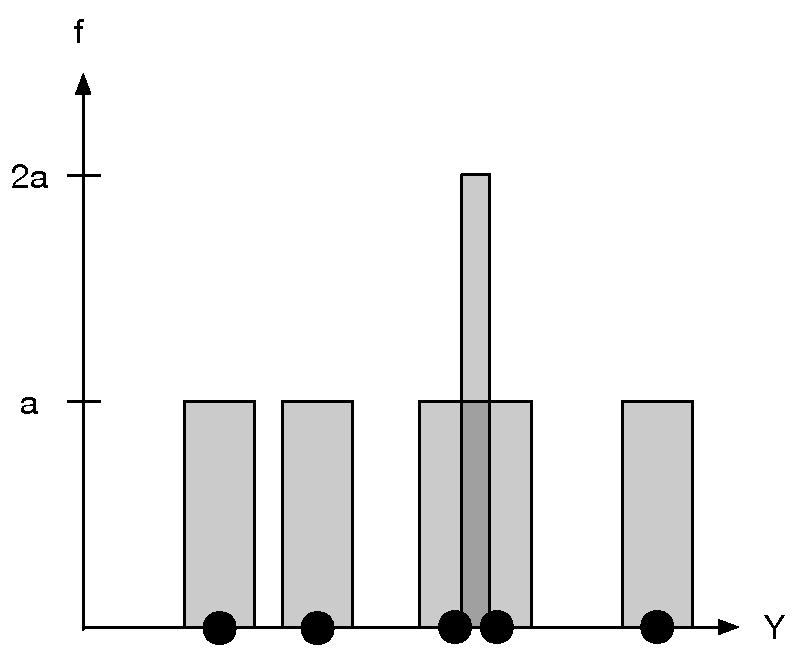
\includegraphics[width=0.6\linewidth,keepaspectratio]{fig/literature/kde.pdf}
\caption{Sketch of a Kernel Density Estimation procedure with a rectangular kernel.}
\label{fig:kde}
\end{figure}

Once the PDF of the QoI is available, it can be used to: \emph{(i)} observe the probability to exceed a threashold; \emph{(ii)} compute the probability to have a certain event; or just \emph{(iii)} get general statistics (mean, variance, quantiles).

\subsection{Sensitivity Analysis}
Sensitivity Analysis (SA) refers to the determination of the contribution of different parameters on quantities of interest~\cite{saltelli2007,iooss2016}. The most natural way to do SA would be to consider the derivatives. But this information is known to be to local or general---although there are some work extending the capabilities of these methods~\cite{kucherenko2016}. In the literature, a distinction is made between local and global SA. In the following, only global-based SA methods are presented with variance-based SA and moment-based SA.

\subsubsection{Variance-based Sensitivity Analysis}\label{sec:sa}
Variance-based Sensitivity Analysis allow to obtain the contribution of the parameters on the QoI's variance~\cite{ferretti2016}. Here, classical \textit{Sobol'}~\cite{Sobol1993} method is presented which gives not only a ranking but also quantifies the importance factor using the variance. This method makes the hypothesis of the independence of the input variables. It uses a functional decomposition of the variance of the function to explore
\begin{align}
\mathbb{V}(Y) &= \sum_{i}^{d} \mathbb{V}_i (Y) + \sum_{i<j}^{d}\mathbb{V}_{ij} + ... + \mathbb{V}_{1,2,...,d},\\
\mathbb{V}_i(Y) &= \mathbb{\mathbb{V}}[\mathbb{E}(Y|x_i)]\nonumber\\
\mathbb{V}_{ij} &= \mathbb{\mathbb{V}}[\mathbb{E}(Y|x_i x_j)] - \mathbb{V}_i - \mathbb{V}_j,\nonumber
\end{align}
\noindent with $p$ the number of input parameters constituting $\mathbf{x}$. This way \textit{Sobol'} indices are expressed as
\begin{align}
S_i = \frac{\mathbb{V}[\mathbb{E}(Y|x_i)]}{\mathbb{V}[Y]}\qquad S_{ij} = \frac{\mathbb{V}[\mathbb{E}(Y|x_i x_j)] - \mathbb{V}_i - \mathbb{V}_j}{\mathbb{V}[Y]}.
\end{align}
\noindent $S_{i}$ corresponds to the first order term which apprises the contribution of the \textit{i-th} parameter, while $S_{ij}$ corresponds to the second order term which informs about the correlations between the \textit{i-th} and the \textit{j-th} parameters. These equations can be generalized to compute higher order terms. However, the computational effort to converge them is most often not at hand and their analysis and interpretations are not simple.

Total indices represents the global contribution of the parameters on the variance of the QoI and express as:
\begin{align}
S_{T_i} = S_i + \sum_j S_{ij} + \sum_{j,k} S_{ijk} + ... = 1 - \frac{\mathbb{V}[\mathbb{E}(Y|x_{\sim i})]}{\mathbb{V}[Y]}.
\end{align}

\Cref{fig:sobol}(b) is an example using \textit{Ishigami} function~\cite{ishigami1990}
\begin{align}
Y(\mathbf{x}) = \sin x_1 + 7 \sin^2 x_2 + 0.1 x_3^4 \sin x_1,
\end{align}
\noindent with $\mathbf{x} \in [-\pi, \pi]^3$. This function exhibits strong nonlinearity and nonmonotonicity. It is particularly interesting because the first order indice of $S_{x_3} = 0$ whereas it's total order is $S_{T_{x_3}} = 0.244$. Note that on second order indices, $S_{x_1,x_3} = 0.244$. It means that almost 25\% of the observed variance on the QoI is due to the correlations between $x_3$ and $x_1$, although $x_3$ by itself has no impact on the QoI.

Looking at \cref{fig:sobol}(a), it can be noted that the convergence of these indices require a large sampling size. The required sampling size is case dependant as it depends on the number of input parameters and on the complexity of the function of interest.

\begin{figure}[H]               
\centering
\subfloat[Convergence of the \emph{Sobol'} indices]{
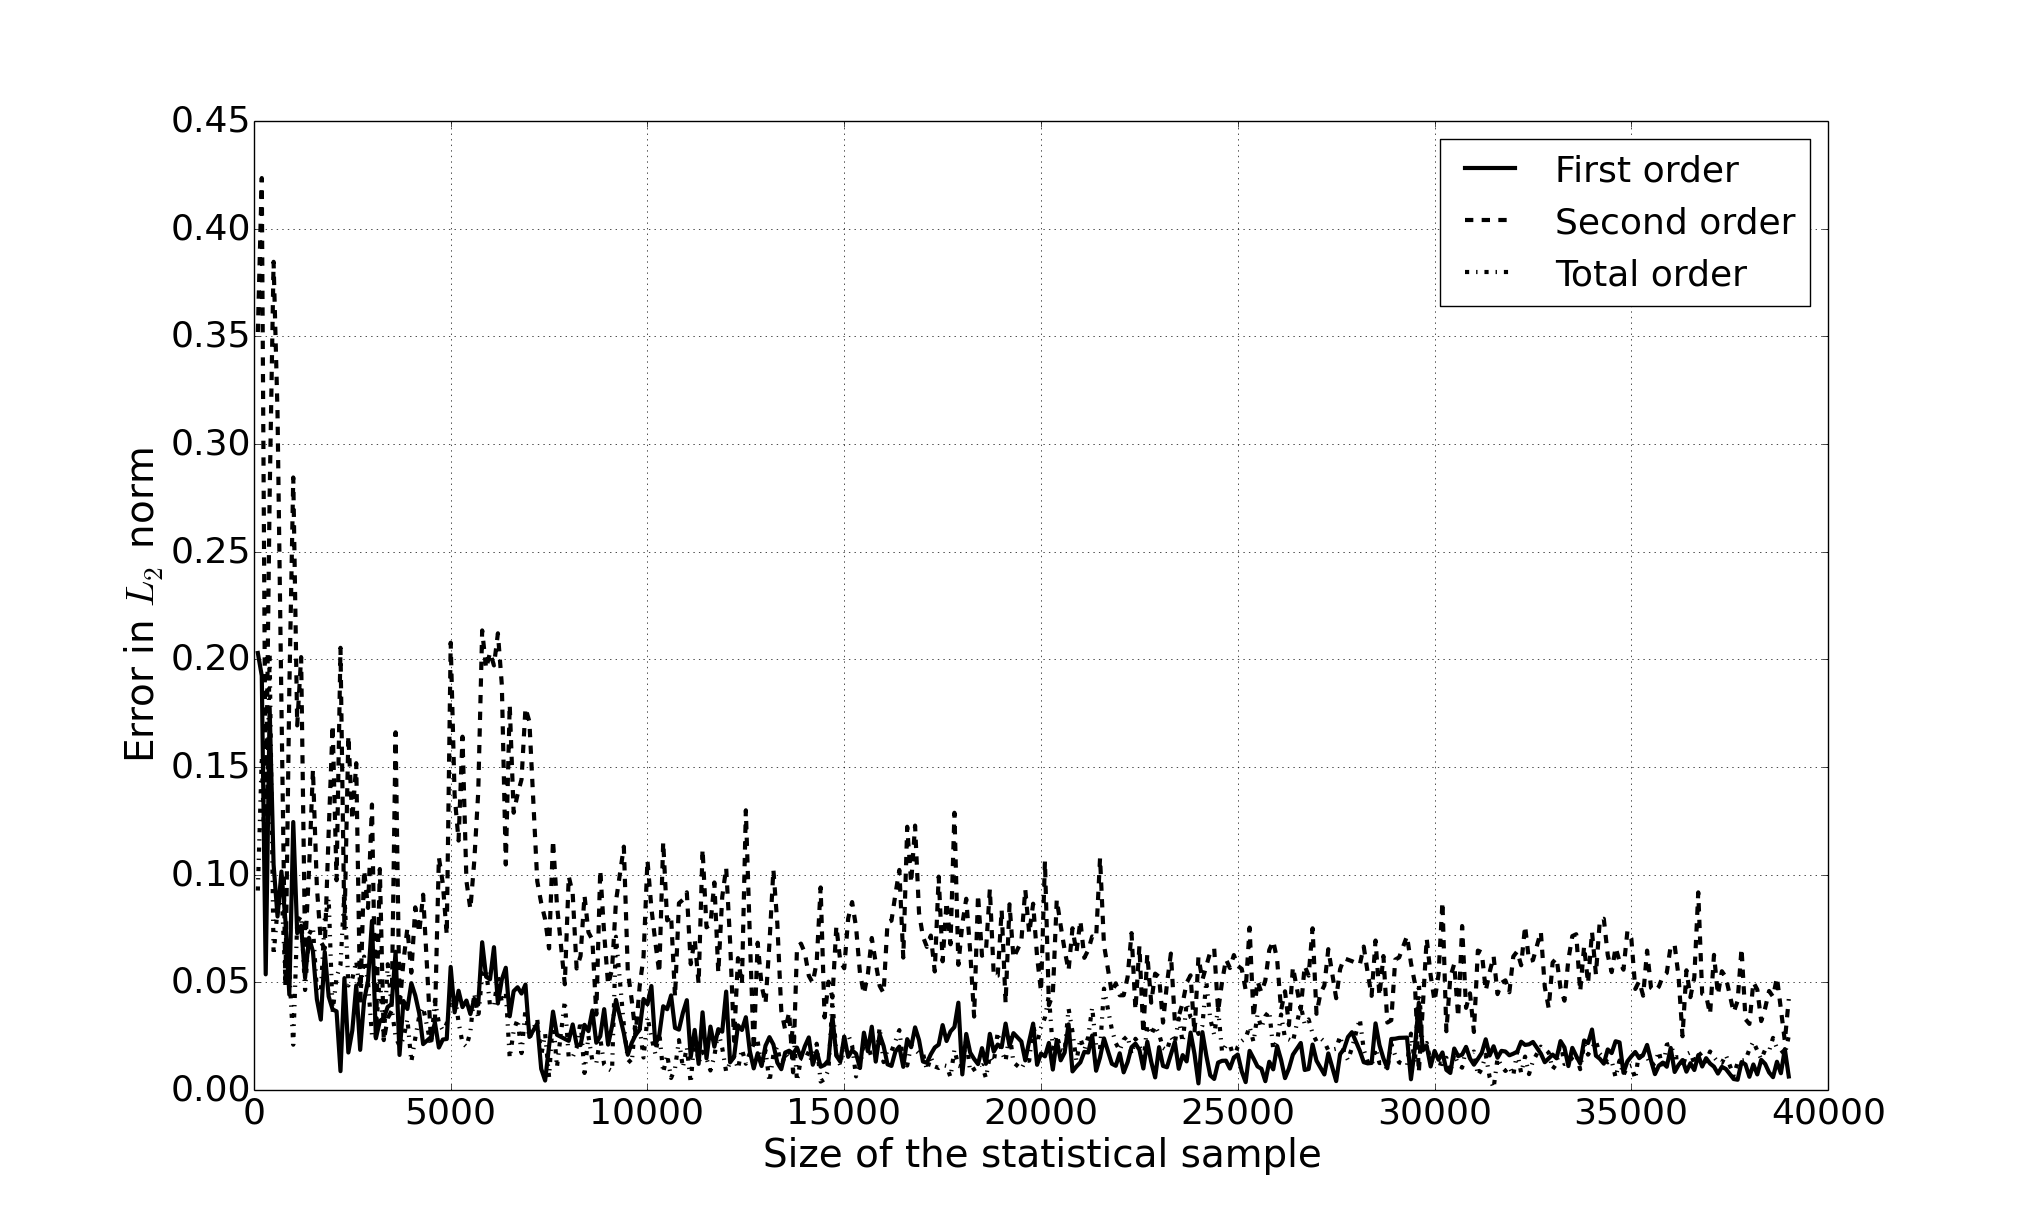
\includegraphics[width=0.47\linewidth,height=\textheight,keepaspectratio]{fig/literature/l2_sample.png}}
 ~       
\subfloat[First and total \textit{Sobol'} indices]{
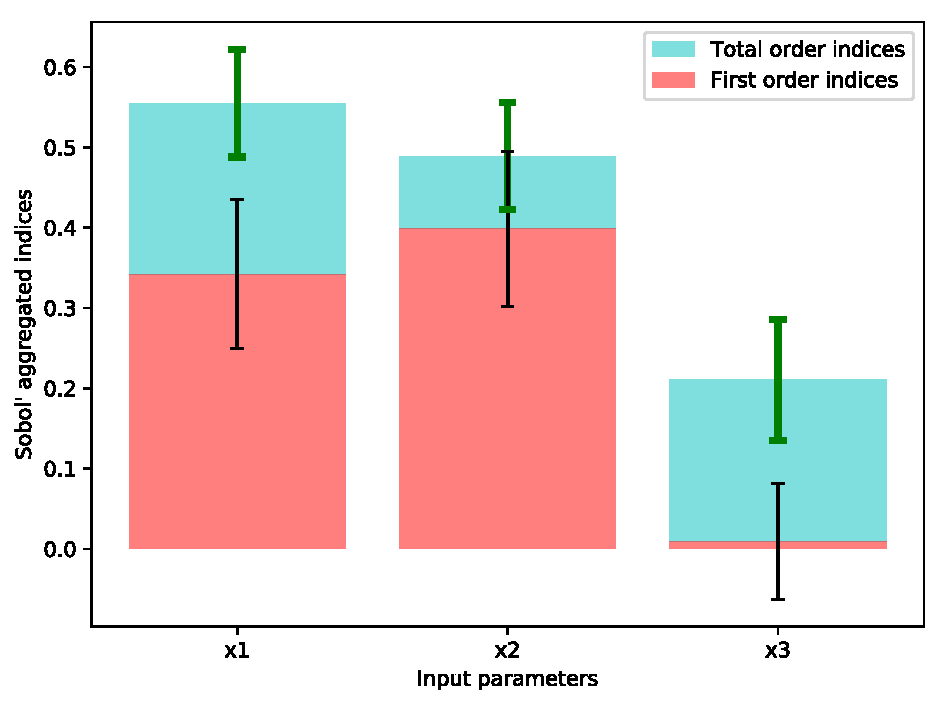
\includegraphics[width=0.47\linewidth,height=\textheight,keepaspectratio]{fig/literature/sobol_aggregated.pdf}}
\caption{First and total \textit{Sobol'} indices on the Ishigami function.}
\label{fig:sobol}
\end{figure}
Classical empirical formulations of \emph{Sobol'} indices require the use of 3 (resp. 4) matrices to compute first and total (resp. and second order indices)~\cite{saltelli2010}. The computation requires two independent sampling $A$, $B$ of size $N$ and a matrice $AB$ which is a combination of both matrices (resp. $BA$). $AB_{n}$ corresponds to the matrice $A$ with the column $n$ from the matrice $B$. Hence the number of forward model evaluation is $N_s = N(d + 2)$. In~\cite{baudin2016}, they showed that \textit{Martinez}' formulation is stable and provides asymptotic confidence intervals---approximated with Fisher's transformation---for first order and total order indices. \textit{Martinez}' estimators write
\begin{align}
\hat{S_i} = \rho (Y(B), Y(AB_{n})) \quad \hat{S_{T_i}} = 1 - \rho (Y(A), Y(AB_n)),
\end{align}
\noindent where $\rho$ is the linear correlation coefficient.

For a functional output, as for the \textit{LS89} blade case---see~\cref{chap:ls89} and \cref{fig:map_sobol}---, \textit{Sobol'} indices can be computed all along the output and retrieve a map or create composite indices. As described by Marrel~\cite{marrel2015}, aggregated indices can also be computed as the mean of the indices weighted by the variance at each point or temporal step
\begin{align}
S_i = \frac{\displaystyle\sum_{l = 1}^{m} \mathbb{V} [\mathbf{Y}^l] S_i^{l}}{\displaystyle\sum_{l = 1}^{m} \mathbb{V} [\mathbf{Y}^l]}.
\end{align}

\begin{figure}[H]
\centering
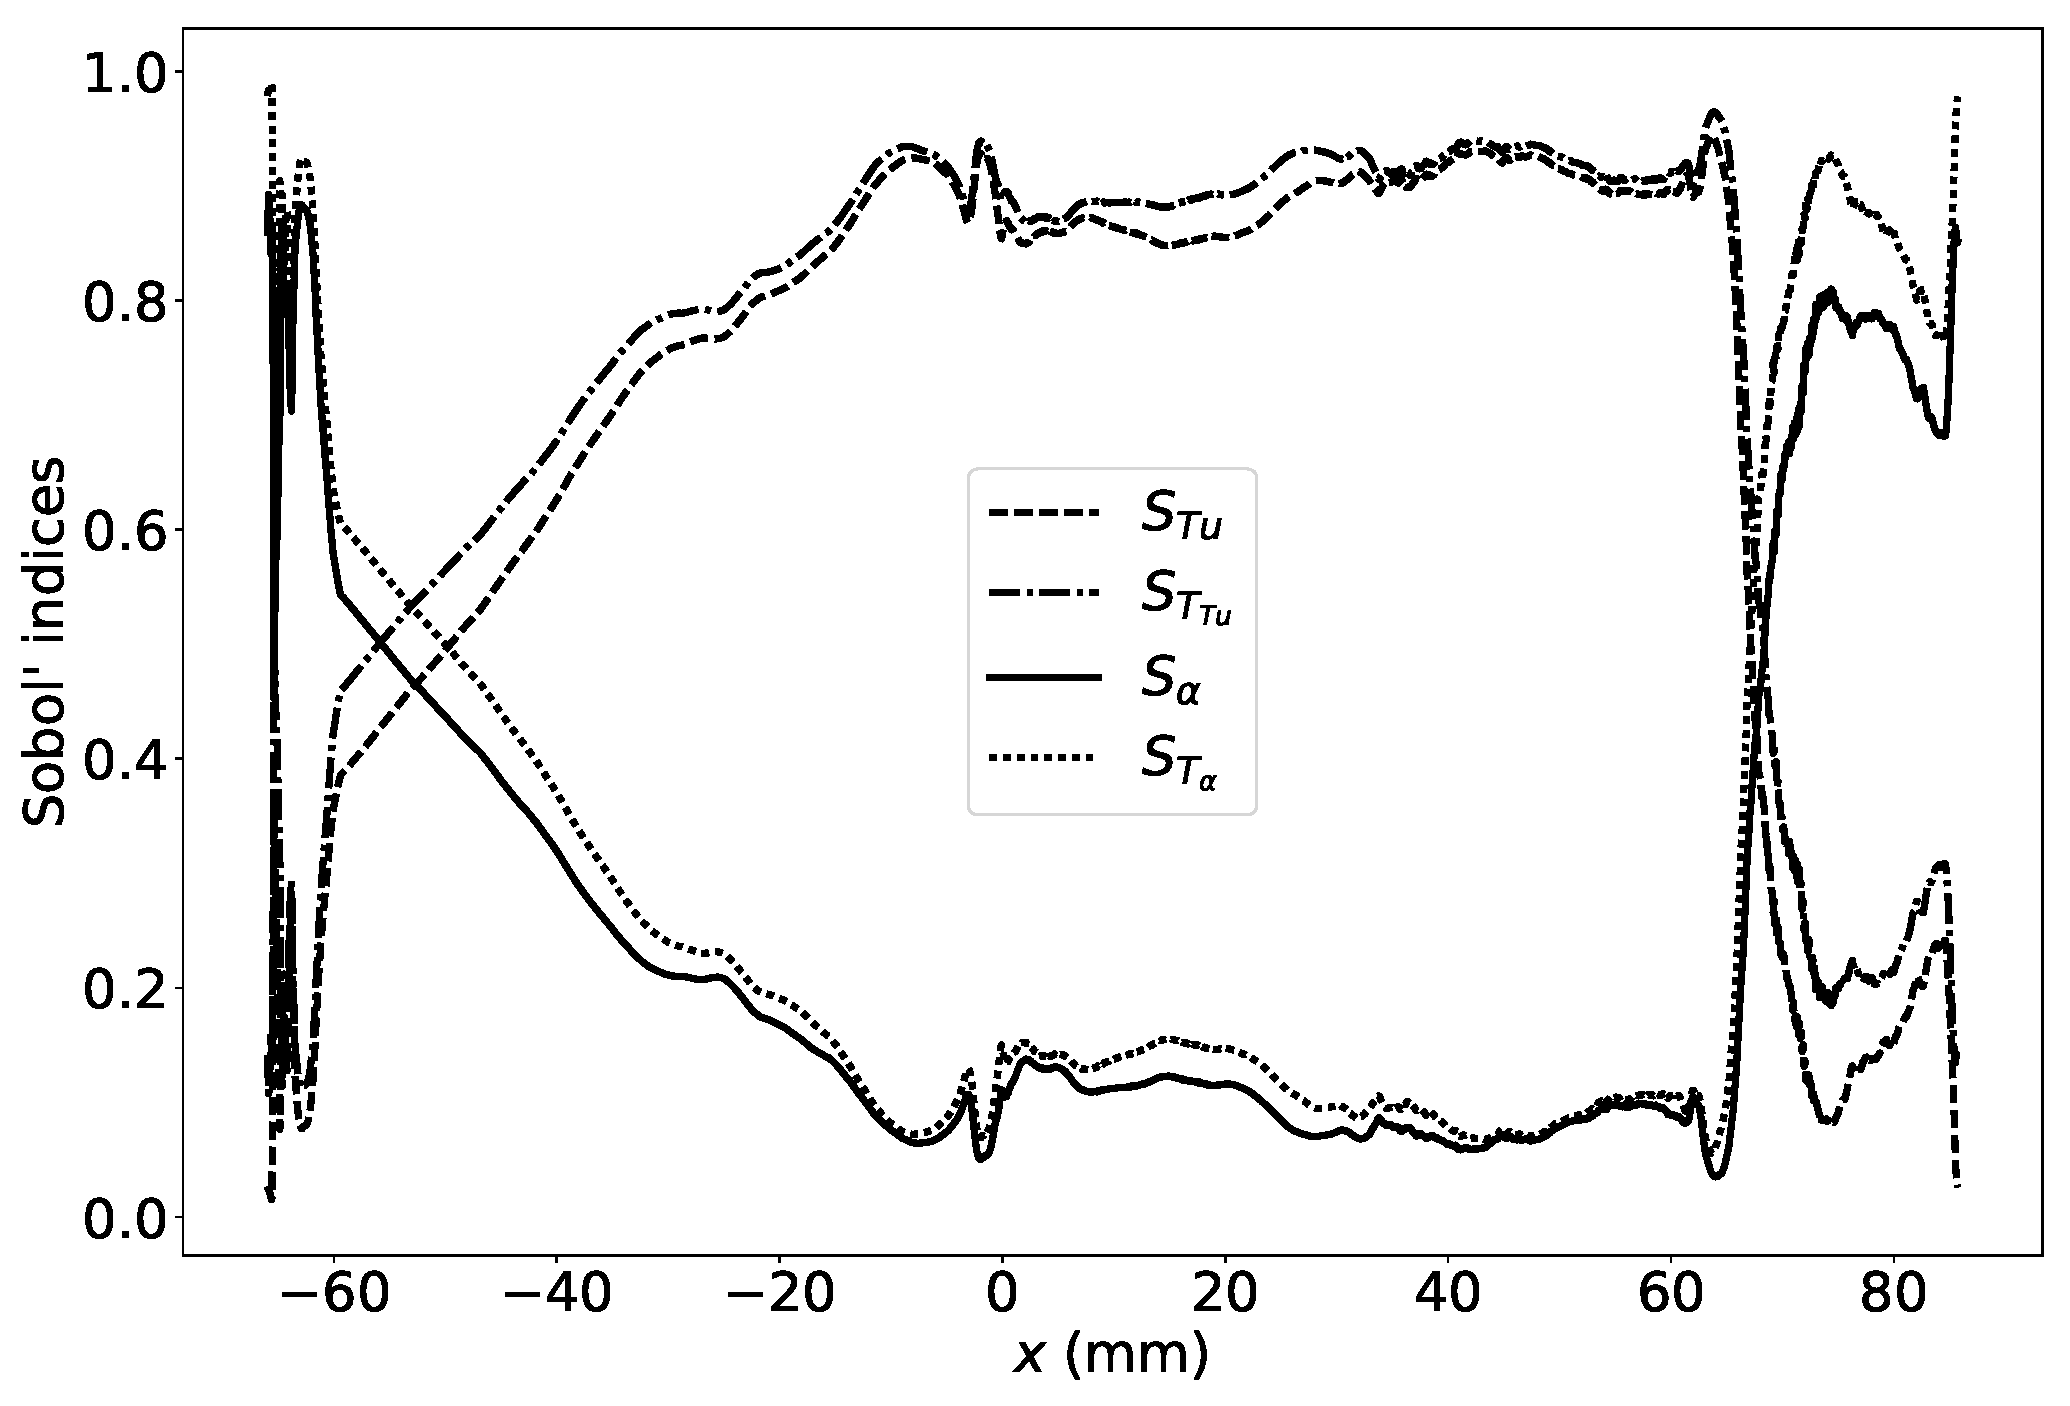
\includegraphics[width=0.8\linewidth,keepaspectratio]{fig/literature/sobol_map.pdf}
\caption{Map of \emph{Sobol'} indices along the \textit{LS89} blade.}
\label{fig:map_sobol}
\end{figure}

\subsubsection{Moment-based Sensitivity Analysis}
Variance-based SA are standard methods (although elementary effects or classical regression are still commonly used among practitioners~\cite{ferretti2016}) but they do not come without flaws~\cite{borgonovo2016}:

\begin{itemize}
\item Only the second order moment is taken into account,\\
It means that if the QoI's PDF is highly skewed, multimodal or with heteroscedastic data, this information will be lost. Hence, the variance is only a good measure if the distribution is close to normal.
\item The parameters need to be uncorrelated,\\
This assumption can be mitigated by using some correlation matrices but the procedure is not really trivial.
\item Null first order indices does not imply that the parameter is independent with the QoI,\\
Computation of high order terms and total effect require a lot of samples to converge. It may be impractical to compute these quantities.
\end{itemize}

Moment-based method are based on the whole PDF to mitigate these issues~\cite{borgonovo2007}. Based on the unconditional PDF, a conditional PDF per parameter is computed. The more the conditional PDF deviates from the unconditional PDF, the more the parameter has an impact on the quantity of interest. The same procedure can be done using the Empirical Cumulative Density Function (ECDF), respectively with the unconditional ECDF. \Cref{fig:moment_sa} shows the computation of both conditional and unconditional PDF (resp. ECDF). Based on these moment estimations, distance criteria can be computed such as: $L_1$, \emph{Kolmogorov-Smirnov} or the \emph{Kuiper} distances. The method does not require any particular sampling nor do not require the parameters to be independent. The limitations comes from the ability to correctly estimate the densities.

\begin{figure}[H]
\centering
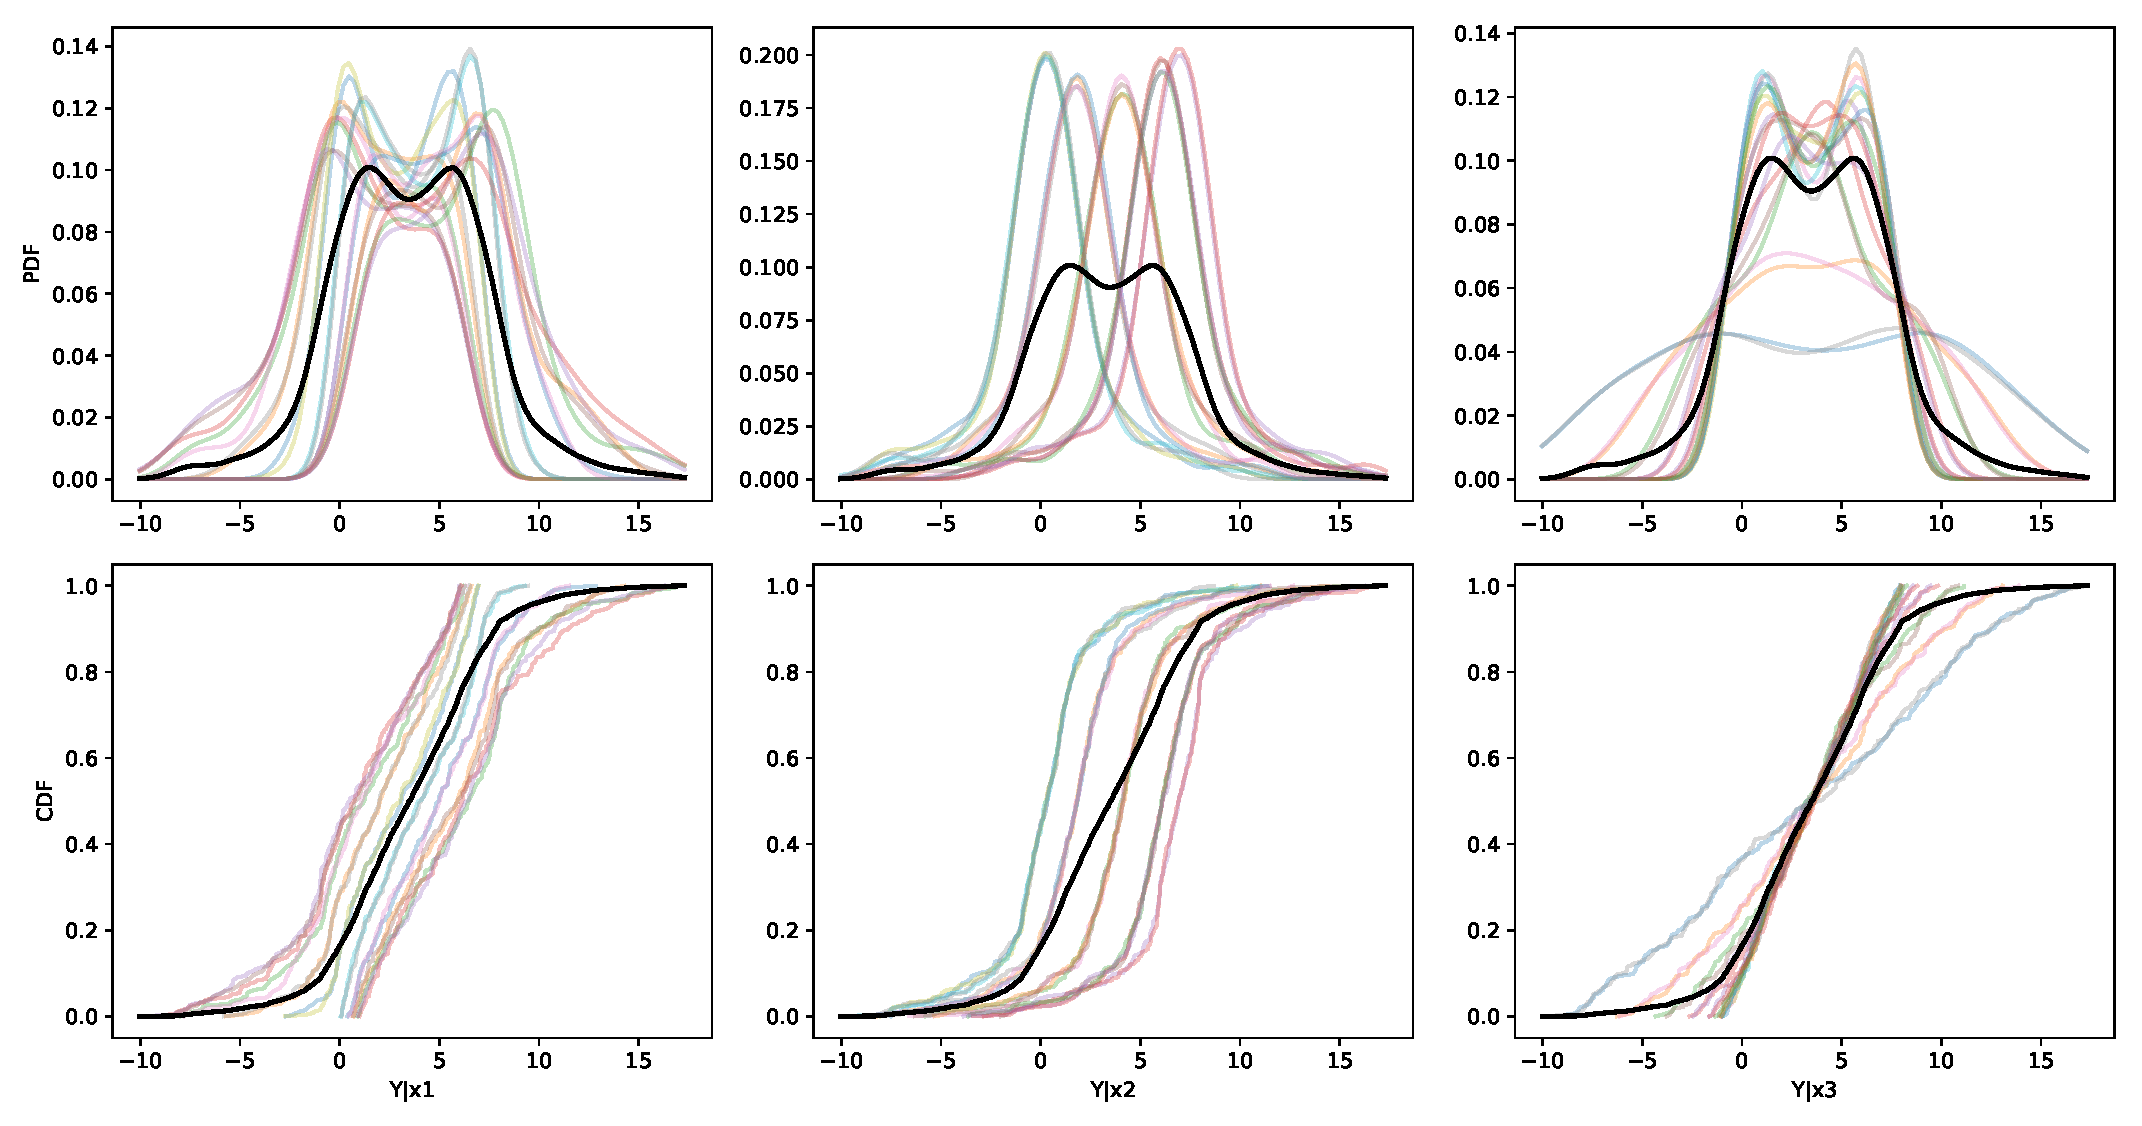
\includegraphics[width=0.8\linewidth,keepaspectratio]{fig/literature/moment_independent-ishigami.pdf}
\caption{Moment independent SA on the \emph{Ishigami} function.}
\label{fig:moment_sa}
\end{figure}

Another visual approach is found with the Cumulative Sums Of NOrmalized Reordered Output method (CUSUNORO)~\cite{Plischke2012}. The output is normalized and ordered in function of a given parameter. Then, its cumulative sum vector is computed. In other words, this corresponds to the conditional ECDF after normalization. Here as well, the more the curve is far from the unconditional ECDF (a flat line after normalization), the more the output is sensitive to the parameter---see~\cref{fig:cusunoro}.

\begin{figure}[H]
\centering
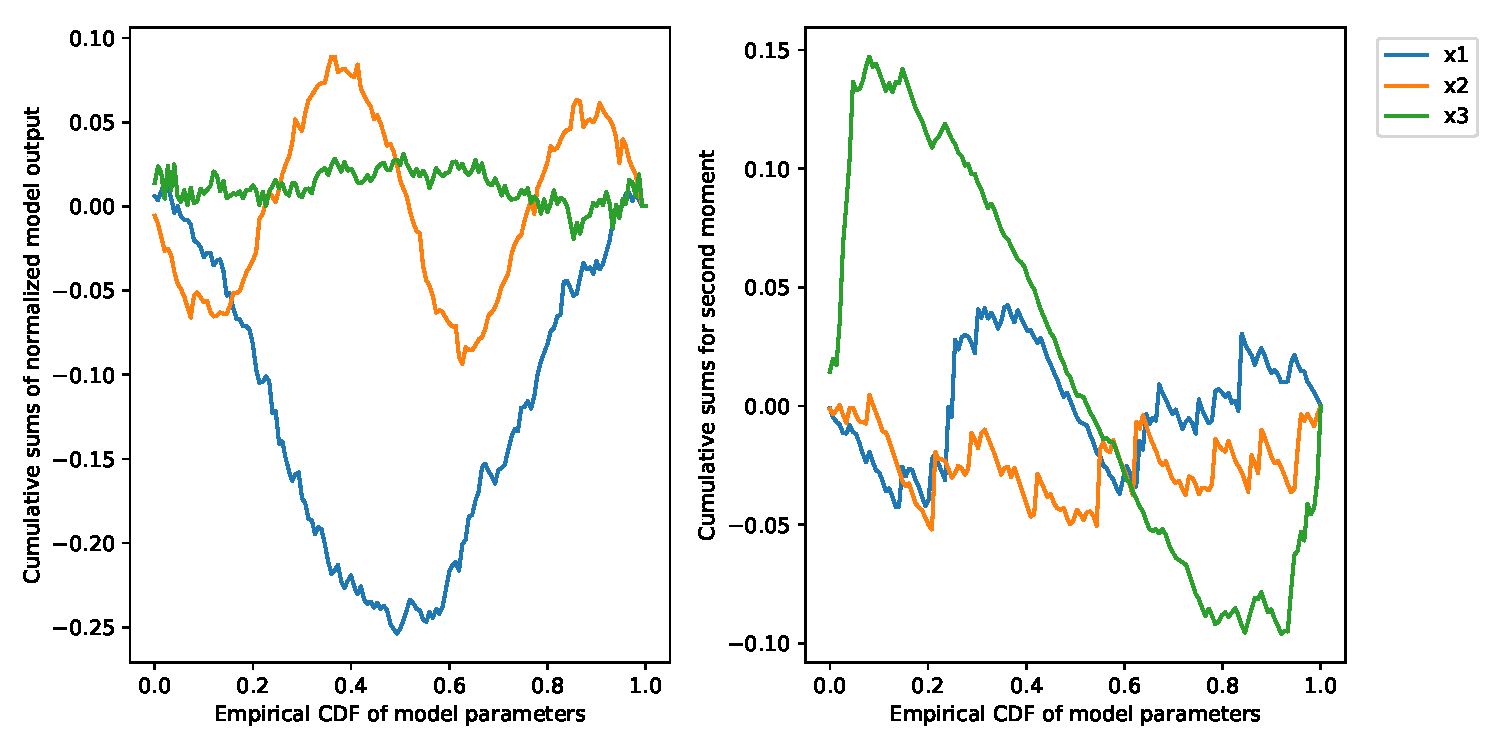
\includegraphics[width=0.8\linewidth,keepaspectratio]{fig/literature/cusunoro-ishigami.pdf}
\caption{CUSUNORO on the \emph{Ishigami} function.}
\label{fig:cusunoro}
\end{figure}


\section{Surrogate Models}\label{sec:surrogate}

Classical UQ methods, based on the Monte-Carlo approach, require a large number of experiments~\citep{iooss2010,iooss2016,lamboni2011,lemaitreknio2010,Saltelli2007,Storlie2009}, which quickly go beyond the limits of available resources (CPU cost, budget). In the following, numerical experiments are considered and especially Computational Fluid Dynamics (CFD) simulations. These limits are especially true when it comes to large dimensional problems, both with respect to the domain discretization and to the number of uncertain input parameters. The cost of the UQ study can, however, be significantly reduced when the CFD code is replaced by a surrogate model which is formulated in a parameter space and which is fast to evaluate for any set of uncertain variables~\cite{martin2005}. Formulating the surrogate model relies on a limited number of forward model integrations referred to as the DoE. Several surrogate models are found in the literature, among whom generalized linear models, polynomial models, splines, polynomial chaos expansions, artificial neural networks or Gaussian process models.

Polynomial chaos (PC) approach has received much attention lately~\citep{dubreuil2014,sudret2008,xiu2010,xiu2002,Ciriello2013}. The PC surrogate model is formulated as a polynomial expansion, in which the basis is defined according to the distribution of the uncertain inputs $\mathbf{x}$ and the coefficients relate to the statistics of the output $\mathbf{Y}$. The coefficients are computed so as to fit the training set $(\mathbf{X}, \mathcal{Y})$, either using regression or spectral projection methods. The merits of PC surrogates were demonstrated in various fields, e.g.~structural mechanics~\citep{dubreuil2014,berveiller2005}, CFD~\citep{hosder2006,lucor2007,saad2007phd}, hydrology~\citep{deman2015}, hydraulics~\citep{ge2008,elmocaydphd}, wildfires~\citep{rochoux2014}. A complementary approach between PC and EnKF was presented in~\citet{lixiu2009} and tested in the framework of wildfire behaviour forecasting in~\citet{rochoux2014}. A PC surrogate was used in place of the forward model to estimate the Kalman gain and thereby design a cost-effective EnKF inferring new estimates of the input parameters (e.g.~biomass moisture and fuel aspect ratio) reducing bias in the fire front location prediction. The resulting algorithm achieved convergence in spite of the non-linear surface response, showing promising results for environmental risk monitoring. 

Gaussian processes (GP) that are strongly related to Kriging in geostatistics also are of increasing interest~\citep{rasmussen2006,legratiet2017,lockwood2012,marrel2015}. The GP formalism treats the forward model response as a realization of a Gaussian stochastic process indexed by $\mathbf{x}$ and fully characterized with mean and covariance functions conditioned by the training set $(\mathbf{X}, \mathcal{Y})$. The GP surrogate is built first, by defining a covariance kernel function between output values and a trend function and then, by estimating the hyperparameters (e.g.~variance, characteristic length scale) that provide a good fit to the training set. GP surrogates were introduced in the context of SA for estimating \emph{Sobol'} indices~\citep{oakley2004,marrel2009,legratiet2014}. In an industrial context---which is the case here---, some benefits of this method are:\textit{(i)} it does not require any prior knowledge on the probability distribution of the uncertainties on the input parameters ; \textit{(ii)} it does not need a specific sampling of the parameter space which could lead to \textit{curse-of-dimensionality} or mis-evaluation of the space ; and \textit{(iii)} it provides an estimation of the predictive error.

PC and GP surrogate models have recently been compared for UQ and SA studies~\citep{legratiet2017,owen2015,schoebi2015}. \citet{owen2015} evaluated the performance of each type of surrogate in terms of output mean, variance and PDF estimation. \citet{legratiet2017} compared \emph{Sobol'} indices with applications in structural mechanics; for a given size of the training set, PC and GP surrogate models were found to feature a similar predictive quality---with respect to the predictive coefficient $Q_2$, also called Nash-Sutcliffe model efficiency coefficient, which is equivalent to the coefficient of determination $R^2$ for residuals' prediction~\citep{krause2005}. \citet{legratiet2017} also emphasized that the ranking between PC and GP approaches remains problem-dependent.

Before going further, let us clarify the nature of the forward model. The ensemble $\mathcal{Y}$ constitute a set of observed QoI. Each element can either be a scalar or a vectorial---or functional---QoI. When considering scalar QoI, a global physical parameter such as the mean temperature for instance, a single surrogate model mapping $Y^{(i)} := \mathcal{M}(\mathbf{x}^{(i)})$ can be constructed. In case of a multidimensional output the mapping comes to $\mathbf{Y}^{(i)} := \mathcal{M}(\mathbf{x}^{(i)})$. One can consider independent surrogate for each element but the computational cost can rapidly become intractable. Moreover, the elements of the vectorial QoI can be correlated. A classical solution is found through the use of a Proper Orthogonal Decomposition (POD)~\cite{anindyachatterjee2000}. By performing a POD on the QoI, each mode being orthogonal, they can be treated as independent and then a surrogate can be built on a reduced space. In~\cite{braconnier2011,margheri2016}, this method was used to reduce the computational cost and conserve the spatial/temporal correlation of the QoI.

Two types of surrogate models are presented in this work to approximate the behaviour of forward models. PC expansion on the one hand, GP regression on the other hand. Considering the general case of a functional QoI, the common idea of PC and GP approaches is to design for each element (with or without considering a POD) $a \in \{a_1, \cdots, a_M\}$ a surrogate with a weighted finite sum of basis functions:
\begin{equation}
\widehat{Y}_a\left(\mathbf{x}\right) = \displaystyle\sum_{i = 0}^{r}\,\gamma_{a,i}\,\Psi_{i}\left(\mathbf{x}\right),
\label{eq:SurrogateForm}
\end{equation}
where the coefficients $\gamma_{a,i}$ and the basis functions $\Psi_i$ are calibrated by the training set $\mathbf{X}^{N_s}$. The main difference between PC (Sect.~\ref{sec:PC}) and GP (Sect.~\ref{sec:GP}) approaches stands in the nature of these models: GP interpolates the training points and captures local variations, while PC is a regression method focusing on the global behaviour of the model. Basis functions and calibration methods also differ between these two approaches.

\Cref{sec:POD} present the POD while \cref{sec:PC} and \cref{sec:GP} respectively define the PC and the GP surrogate methods.

%For PC expansion, the maximum order of the decomposition and the basis functions are first chosen, then a spectral projection strategy is implemented to compute the decomposition coefficients in the polynomial basis. The GP strategy is two-fold: the first step consists in transforming the sampled output space to an orthogonal one, eventually reducing its dimension; the second step consists in interpolating with a GP approach the principal components of this new space to express water level in the basis for any friction and discharge values. It should be noted that the GP model could be replaced by any other interpolator. 

\subsection{Snapshot method}\label{sec:POD}

% TODO indices or not?

The key idea of the snapshot method~\citep{sirovich1987} is to achieve a POD of the centred snapshot matrix $\mathcal{Y} \in \mathbb{M}_{M,N}(\mathbb{R})$, which gathers the discretized QoI for the $N_{s}$ snapshots, from which the sample mean is subtracted. For simplicity purpose, the QoI anomaly element $a$ is denoted $y$ in the following. Thus, $\mathcal{Y} = \left(y_{a_i}^{(j)}\right)_{1\leq i \leq M \atop 1\leq j \leq N_{s}}$. The snapshots correspond to the column vectors; the $k$th snapshot of size $M$ is denoted by $\mathbf{y}^{(k)}$.

Based on many observations of a random vector, the POD gives the orthogonal directions of largest variances (or modes) in the probabilistic vector space in order to reduce the vector space dimension~\citep{chatterjee2000}. Note that for simplicity purpose, the adjective {\it centred} is dropped in the following when referring to the centred snapshot matrix $\mathcal{Y}$.

The POD of the snapshot covariance matrix $\mathbf{C} = N_{s}^{-1}\,\mathcal{Y}^{\mathrm{T}}\,\mathcal{Y}\in \mathbb{M}_{N_{s}}(\mathbb{R})$ is equivalent to the Singular Value Decomposition (SVD) of the snapshot matrix $\mathcal{Y}$:
\begin{equation}
\mathcal{Y} = \mathbf{U}\,\mathbf{\Lambda}\,\mathbf{V}^{\mathrm{T}} = \displaystyle\sum_{k = 1}^{r_{p}}\,\lambda_k\,\mathbf{u}_k\,\mathbf{v}_k^{\mathrm{T}},
\end{equation} 
where $\mathbf{U} \in \mathbb{M}_M(\mathbb{R})$ is an orthogonal matrix diagonalizing $\mathcal{Y}\mathcal{Y}^{\mathrm{T}}$ ($\mathbf{u}_k$, the $k$th column of $\mathbf{U}$, is a left singular vector of $\mathcal{Y}$), where $\mathcal{V} \in \mathbb{M}_N(\mathbb{R})$ is an orthogonal matrix diagonalizing $\mathcal{Y}^{\mathrm{T}}\mathbf{Y}$ ($\mathbf{v}_k$, the $k$th column of $\mathbf{V}$, is a right singular vector of $\mathcal{Y}$), and where $\mathbf{\Lambda} \in \mathbb{M}_{M,N_{s}}(\mathbb{R})$ is a rectangular diagonal matrix including $r_{p}=\min(M,N_{s})$ singular values on its diagonal. The singular values $\lbrace \lambda_k \rbrace_{1 \leq k \leq r_{p}}$ are the square roots of the eigenvalues of $\mathbf{C}$. 
Note that in this study, we do not reduce further the rank of the snapshot matrix $\mathcal{Y}$. %Since the number of stations ($M = 14$) is lower than the size of the training set $N$, the rank of $\mathbf{Y}$ is here $r_{p} = M$.

For a given element $a$, any snapshot $h_a(\mathbf{x}^{(k)})$ can then be retrieved as a linear combination of $r_{p}$ modes $\{\Psi_i\}_{1\leq i \leq r_p}$:
\begin{equation}\label{eq:gppod}
y_a(\mathbf{x}^{(k)}) 
= (\mathbf{U}\,\mathbf{\Lambda}\,\mathbf{V}^{\mathrm{T}})_{ak} 
= U_{a:}(\mathbf{\Lambda}\,\mathbf{V}^T)_{:k}=\sum_{i=1}^{r_{p}}\,\gamma_{a,i}\,\Psi_i(\mathbf{x}^{(k)}),
\end{equation}
where for any $i\in\{1,\ldots,M\}$, $\gamma_{a,i}:=U_{a,i}$ and $\Psi_i(\mathbf{x}^{(k)}):=(\boldsymbol{\Lambda}\mathbf{V}^T)_{i,k}$. 
%
%In the present study, the size of the state vector $M$ is smaller than the size of the training set $N$, implying that there are $r_p = M$ non-zero singular values. This is usually not the case, but this does not change the methodology. As the objective is to compare PC and pGP and as there is a limited number of stations $M$, all modes are kept to avoid the loss of information, there is no need to reduce the rank of the singular matrix. Note that when moving to 2-D or 3-D cases (beyond the scope of the present work), the size of the state vector could be of the order of thousands components, making dimension reduction necessary. 


%----Polynomial Chaos
\subsection{Polynomial Chaos (PC) surrogate model}\label{sec:PC}

The algorithm to build the PC surrogate proceeds as follows:
\begin{enumerate}
\item choose the polynomial basis $\lbrace\Psi_{i}\rbrace_{i\geq 0}$ according to the assumed PDF of the inputs $\mathbf{x}$,
\item choose the total polynomial degree $P$ according to the complexity of the physical processes,
\item truncate the expansion to $r_{\text{pc}}$ terms to keep the predominant information given by the forward model using standard truncation strategy ($r_{\text{pc}}$ depends on $d$ and $P$),
\item apply spectral projection strategy (i.e.~Gaussian quadrature rule) to compute the coefficients $\lbrace\gamma_{a,i}\rbrace_{i\in\mathbb{N}^d\atop|i|\leq P}$ for each element $a$ (can use a POD or not) using $N_{s} = (P+1)^{d}$ snapshots,
\item formulate the surrogate model $\mathcal{M}_{\text{pc}}$ at each element $a$, which can be evaluated for any new pair of parameters $\mathbf{x}^*$.
\end{enumerate}
Note that we use standard truncation and projection strategies presented in~\cite{lemaitreknio2010} and \cite{xiu2010}.

\subsubsection{Polynomial basis}

Each component of the random vector $\mathbf{x}$ defined in the input physical space is standardized and noted $\boldsymbol{\zeta}$ in the following way: $\zeta_i=\frac{x_i-\mu_i}{\sigma_i}$ where $\mu_i=N_{s}^{-1}\sum_{k=1}^{N_{s}}x_i^{(k)}$ and $\sigma_i=\sqrt{(N_{s}-1)^{-1}\sum_{k=1}^{N_{s}}\left(x_i^{(k)}-\mu_i\right)^2}$. 

%Assuming that the SWE solution is of finite variance, each component $h_a$ of the water level vector $\mathbf{h}$ can be considered as a random variable for which there exists a polynomial expansion of the form~\eqref{eq:SurrogateForm} that represents how the water level $h_a$ varies according to changes in $Q$ and $K_{s_3}$. 

$y_a$ is projected onto a stochastic space spanned by the orthonormal polynomial functions $\lbrace\Psi_{i}\rbrace_{i\geq 0}$. These functions are orthonormal with respect to the joint density $\rho(\boldsymbol{\zeta})$, i.e.
\begin{equation}
\int_{Z}\,\Psi_i(\boldsymbol{\zeta})\,\Psi_j(\boldsymbol{\zeta})\,\rho(\boldsymbol{\zeta})\,\mathrm{d}\boldsymbol{\zeta} = \delta_{ij},
\label{eq:pc_innerproduct}
\end{equation}
with $\delta_{ij}$ the Kronecker delta function and $Z \subseteq \mathbb{R}^d$ the space in which $\boldsymbol{\zeta}$ evolves. In practice, the orthonormal basis is built using the tensor product of 1-D polynomial functions: $\Psi_i=\Psi_{i,1}\ldots\Psi_{i,d}$ where $i$ is the multi-index $(i_1,\ldots,i_d)\in\{0,1,\cdots,P\}^d$. The choice for the basis functions depends on the probability measure of the random variables. According to Askey's scheme, the Hermite polynomials form the optimal basis for random variables following the standard Gaussian distribution, and the Legendre polynomials are the counterpart for the standard uniform distribution~\citep{xiu2002}. 

\subsubsection{Truncation Strategy}

In practice, the sum in Eq.~\eqref{eq:SurrogateForm} is truncated to a finite number of terms $r_{\text{pc}}$. Using a standard truncation strategy $r_{\text{pc}}$ is constrained by the number of random variables $d$ and by the total polynomial degree $P$ as:
\begin{equation}
r_{\text{pc}} = \frac{(d + P)!}{d!\,P!},
\label{eq:pc_order}
\end{equation}
meaning that all polynomials involving the $d$ random variables of total degree less or equal to $P$ are retained in the PC expansion. The PC approximated the QoI at each element $y_{\text{pc}}(a)$ is formulated as:
\begin{equation}
\widehat{y}_{\text{pc},a}(\mathbf{x}) := \mathcal{M}_{\text{pc},a}(\boldsymbol{\zeta}) = \displaystyle\sum_{i\in\mathbb{N}^d\atop|i|\leq P}\,\gamma_{a,i}\,\Psi_i\left(\boldsymbol{\zeta}\right).
\label{eq:SurrogatePC}
\end{equation}
Note that for small $d$, advanced truncation strategies that consist in eliminating high-order interaction terms or using sparse structure~\citep{blatman2009phd,migliorati2013} are not necessary.

\subsubsection{Spectral projection strategy}

We focus here on non-intrusive approaches to numerically compute the coefficients $\lbrace\gamma_{a,i}\rbrace_{i\in\mathbb{N}^d\atop |i|<P}$  in Eq.~\eqref{eq:SurrogatePC} using $N_{s}$ snapshots from $\mathbf{X}^{N_s}$. The spectral projection relies on the orthonormality property of the polynomial basis. The $i$th coefficient $\gamma_{a,i}$ is computed using Gaussian quadrature as:
\begin{equation}
\gamma_{a,i} = <y_a,\Psi_i> \,\cong\,\displaystyle\sum_{k = 1}^{N_{s}}\,y_a^{(k)}\,\Psi_i(\boldsymbol{\zeta}^{(k)})\,w^{(k)},
\label{eq:pc_quadrature}
\end{equation}
where $\mathbf{y}^{(k)} = \mathcal{M}(\mathbf{x}^{(k)})$ is the snapshot corresponding to the $k$th quadrature root $\mathbf{x}^{(k)}$ of $\Psi_i$ (in the physical space), and where $w^{k}$ is the weight associated with $\mathbf{x}^{(k)}$. $(P+1)$ is the number of quadrature roots required in each uncertain direction to ensure an accurate calculation of the integral $<y_a,\Psi_i>$. Hence, $N_{s} = (P+1)^2$.


%----Gaussian process
\subsection{Gaussian Process surrogate}\label{sec:GP}

The algorithm to build a Gaussian Process surrogate relies on a POD and proceeds as follows:
\begin{enumerate}
\item choose the size of the training set $N$,
\item draw $N$ samples (or snapshots) in the input random space $\mathbf{x}$,
\item formulate the centred snapshot matrix $\mathbf{Y}$ from the $N$ water level snapshots,
\item achieve a POD on $\mathbf{Y}$ using the snapshot method to derive the basis vectors $\lbrace\Psi_{i}\rbrace$ and the corresponding coefficients $\lbrace\gamma_{a,i}\rbrace$ (any snapshot can be expressed as a linear combination of the basis vectors and coefficients),
\item replace each basis vector $\lbrace\Psi_i\rbrace$ associated to the $N_{s}$ snapshots by a basis function via Gaussian Process regression for any $\mathbf{x}^*$, 
\item formulate the surrogate model $\mathcal{M}_{\text{gp}}$ for the QoI at each curvilinear abscissa $a$, which can be evaluated for any $\mathbf{x}^*$.
\end{enumerate}
Note that we follow the choices made by~\cite{braconnier2011}. 

\subsubsection{Regression Procedure}\label{sec:regression}

Our objective is now to generalize the data set $\lbrace\Psi_i(\mathbf{x}^{(k)})\rbrace_{1\leq k \leq N}$ associated with the design of experiments $\mathcal{X}$ to any new input vector $\mathbf{x}^*$, in order to approximate the model output $h_a$ at any curvilinear abscissa $a$. We thus propose the following surrogate model based on GP regression and Eq.~\eqref{eq:gppod}:
\begin{equation}\label{pgpak}
\widehat{h}_{\text{pgp},a}(\mathbf{x}^*) = \sum_{i=1}^{r_{p}}\gamma_{a,i}\,\Psi_{\text{gp},i}(\mathbf{x}^*),
\end{equation}
where $\Psi_{\text{gp},i}$ is a GP model calibrated from the training set $\left\{\mathbf{x}^{(k)},\Psi_i(\mathbf{x}^{(k)})\right\}_{1\leq k \leq N}$ as detailed in the following. 

As stated by~\citet{rasmussen2006}, a GP is a random process (here the mode $\Psi_i$) indexed over a domain (here $\mathbb{R}^d$), for which any finite collection of process values (here $\left\{\Psi_i(\mathbf{x}^{(k)})\right\}_{1\leq k \leq N}$) has a joint Gaussian distribution. Concretely, let $\widetilde{\Psi}_i$ be a Gaussian random process fully described by its zero mean and its correlation $\pi_i$:
\begin{equation}
\widetilde{\Psi}_i(\mathbf{x})\sim \text{GP}\left(0, \sigma_i^2\,\pi_i(\mathbf{x},\mathbf{x}')\right),
\end{equation}
with $\pi_i(\mathbf{x},\mathbf{x}') = \mathbb{E}\left[\widetilde{\Psi}_i(\mathbf{x})\widetilde{\Psi}_i(\mathbf{x}')\right]$. In our case, the correlation function $\pi$ (or kernel) is chosen as a squared exponential:
\begin{equation}
\pi_i(\mathbf{x}, \mathbf{x}') = \exp\left(-\frac{\|\mathbf{x} - \mathbf{x}'\|^2}{2\,\ell_i^2}\right),
\end{equation}
where $\ell_i$ is a length scale describing dependencies of model output between two input vectors $\mathbf{x}$ and $\mathbf{x}'$, and where $\sigma_i^2$ is the variance of the output signal. Squared exponential kernel leads to satisfying results but other kernel functions could have been considered, such as a decreasing exponential one or a Matérn one -- with their associated hyper-parameters. The choice of the kernel is still an open problem and can be mitigated using the available information on the problem. The square exponential kernel leads to very smooth, thus stable results. Furthermore, it implies that the model is exact at sample points; it does not introduce any other strong assumptions, hence its wide usage among practitioners.

Then the surrogate model of interest is the mean of the GP resulting of conditioning $\widetilde{\Psi}_i$ by the training set $\left\{\Psi_i\left(\mathbf{x}^{(k)}\right)\right\}_{1\leq k \leq N}$. For any $\mathbf{x}^*\in\mathbb{R}^d$,
\begin{equation}
\Psi_{\text{gp},i}(\mathbf{x}^*)=\sum_{k = 1}^N\,\beta_{k,i}\,\pi_i\left(\mathbf{x}^*,\mathbf{x}^{(k)}\right),
\end{equation}
where $\beta_{k,i} = \left(\mathbf{\Pi}_i +\tau^2\,\mathbf{I}_N\right)^{-1}\left(\Psi_i\left(\mathbf{x}^{(1)}\right)\ldots \Psi_i\left(\mathbf{x}^{(N)}\right)\right)^T$ with $\mathbf{\Pi}_i=\left(\pi_i\left(\mathbf{x}^{(j)},\mathbf{x}^{(k)}\right)\right)_{1\leq j,k \leq N}$, and where $\tau$ (referred to as the nugget effect) avoids ill-conditioning issues for the matrix $\mathbf{\Pi}$. The hyperparameters $\left\{\ell_i, \sigma_i, \tau\right\}$ are optimized by maximum likelihood applied to the data set $\mathcal{D}_N$ using a basin hopping technique~\citep{wales1997}.



\section{Uncertainty Visualization}



\section{Software}



\chapter{Scientific Questions}


\section{How to Construct a DoE in a High Dimensional Parameter Space?}

\section{How to Resample a DoE by Considering the Output?}

\section{How to Visualize Uncertainties in High Dimensional Cases?}
